\documentclass{beamer}

% packages
\usepackage[utf8]{inputenc}
\usepackage{graphicx}
\usepackage{indentfirst}
\usepackage{amsmath}
\usepackage{geometry}
\usepackage{amsthm}
\usepackage{amssymb}
\usepackage{graphicx}
\usepackage{float}
\usepackage{setspace}
\usepackage{booktabs}
\usepackage{tabularx,colortbl}
%\usepackage[colorlinks=true,linkcolor=black]{hyperref}
\usepackage{fancyhdr}
%\pagestyle{fancy}
\usepackage{textcomp}
\usepackage{setspace}
\usepackage{lineno}

% more vissulize in introduction 
%  Talk about $\beta$ diversity 
%  more general picture
%  donot show trace
%  why I set the parameter
%  explain what does it mean finding this or that result, should be much simpler
%  make it more ecology

% theme
\usetheme{Ilmenau}
\usecolortheme{beaver}


\title{Spatial Explicit Occupancy Modeling of Mammal Community Using Markov Random Field with Imperfect Observations}
\author{MS Entrance of \\Yunyi SHEN}
\institute{UW Madison\\ Department of Forest and Wildlife Ecology}
\date{\today}

\begin{document}
\frame{\titlepage}
\frame{\tableofcontents}

\section{Introduction}
\begin{frame}{Introduction}
	\begin{itemize}
		\item Island System
		\item Markov Random Field
	\end{itemize}
\end{frame}
\subsection{Island System} 
\begin{frame}{Island Biogeography}
	\begin{columns}
		\column{.5\textwidth}
		\begin{block}{R.H. McArthur}
			\begin{figure}[ht]
				\centering
				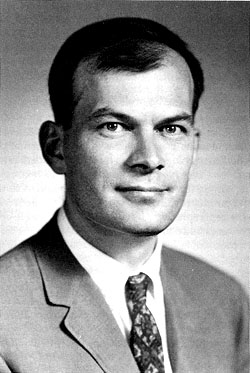
\includegraphics[scale=0.8]{fig/APIS/MacArthur.jpg}
				%\caption{}
				\label{R.H. McArthur}
			\end{figure}
		\end{block}
		
		\column{.5\textwidth}
		\begin{block}{E.O. Wilson}
			\begin{figure}[ht]
				\centering
				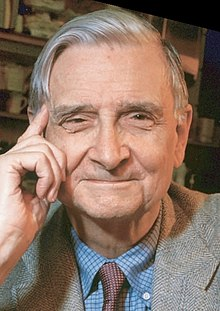
\includegraphics[scale=0.46]{fig/APIS/Wilson.jpg}
				%\caption{Wilson}
				\label{E.O. Wilson}
			\end{figure}
		\end{block}
	
	\end{columns}

\end{frame}





\begin{frame}{Equilibrium Theory of Island Biogeography}
\begin{columns}[c]
	\column{6cm}
	\begin{figure}[ht]
		\centering
		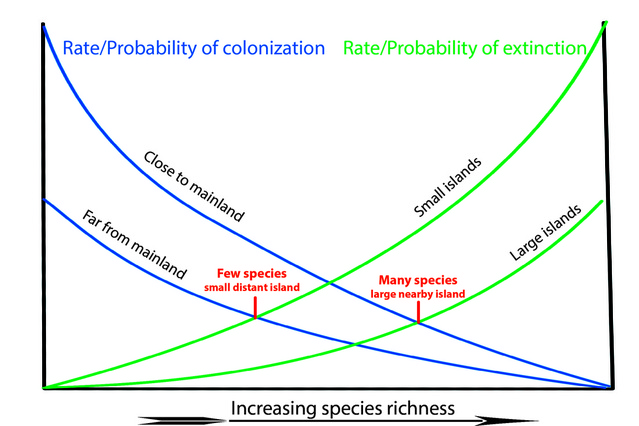
\includegraphics[scale=1.2]{fig/APIS/IBT.jpg}
		%\caption{Wilson}
		\label{IBT}
	\end{figure}
	
	\column{6cm}
	\begin{itemize}
		\item Richness of Island is Equilibrium between: 
		\begin{itemize}
			\item \textbf{Dispersion}
			\item \textbf{Extinction}
		\end{itemize}
		\item Island as single individual
		\item Inter-island relationships
	\end{itemize}
\end{columns}
\end{frame}



\begin{frame}{Mean Field Approximation of Islands}
	\begin{itemize}
		\item Ignore shape of island
		\item Ignore dispersion limit on island\pause
		\item Is it appropriate? \\Context dependent!
	\end{itemize}
\end{frame}

\begin{frame}{Three Interesting Spatial Scales}
\begin{columns}
	\column{5cm}
	\begin{itemize}
		\item[1] Inter island distance
		\item[2] Island length 
		\item[3] Dispersion/homerange
	\end{itemize}
	%I want a map here 
	\column{5cm}
	\begin{itemize}
		\item $1\simeq2$: Shape effect
		\item $2\simeq3$: Intra island structure
	\end{itemize}
	%I want a fox here
\end{columns}
\end{frame}

\begin{frame}{Apostle Islands} % talk about specific speices.
	\begin{figure}[ht]
		\centering
		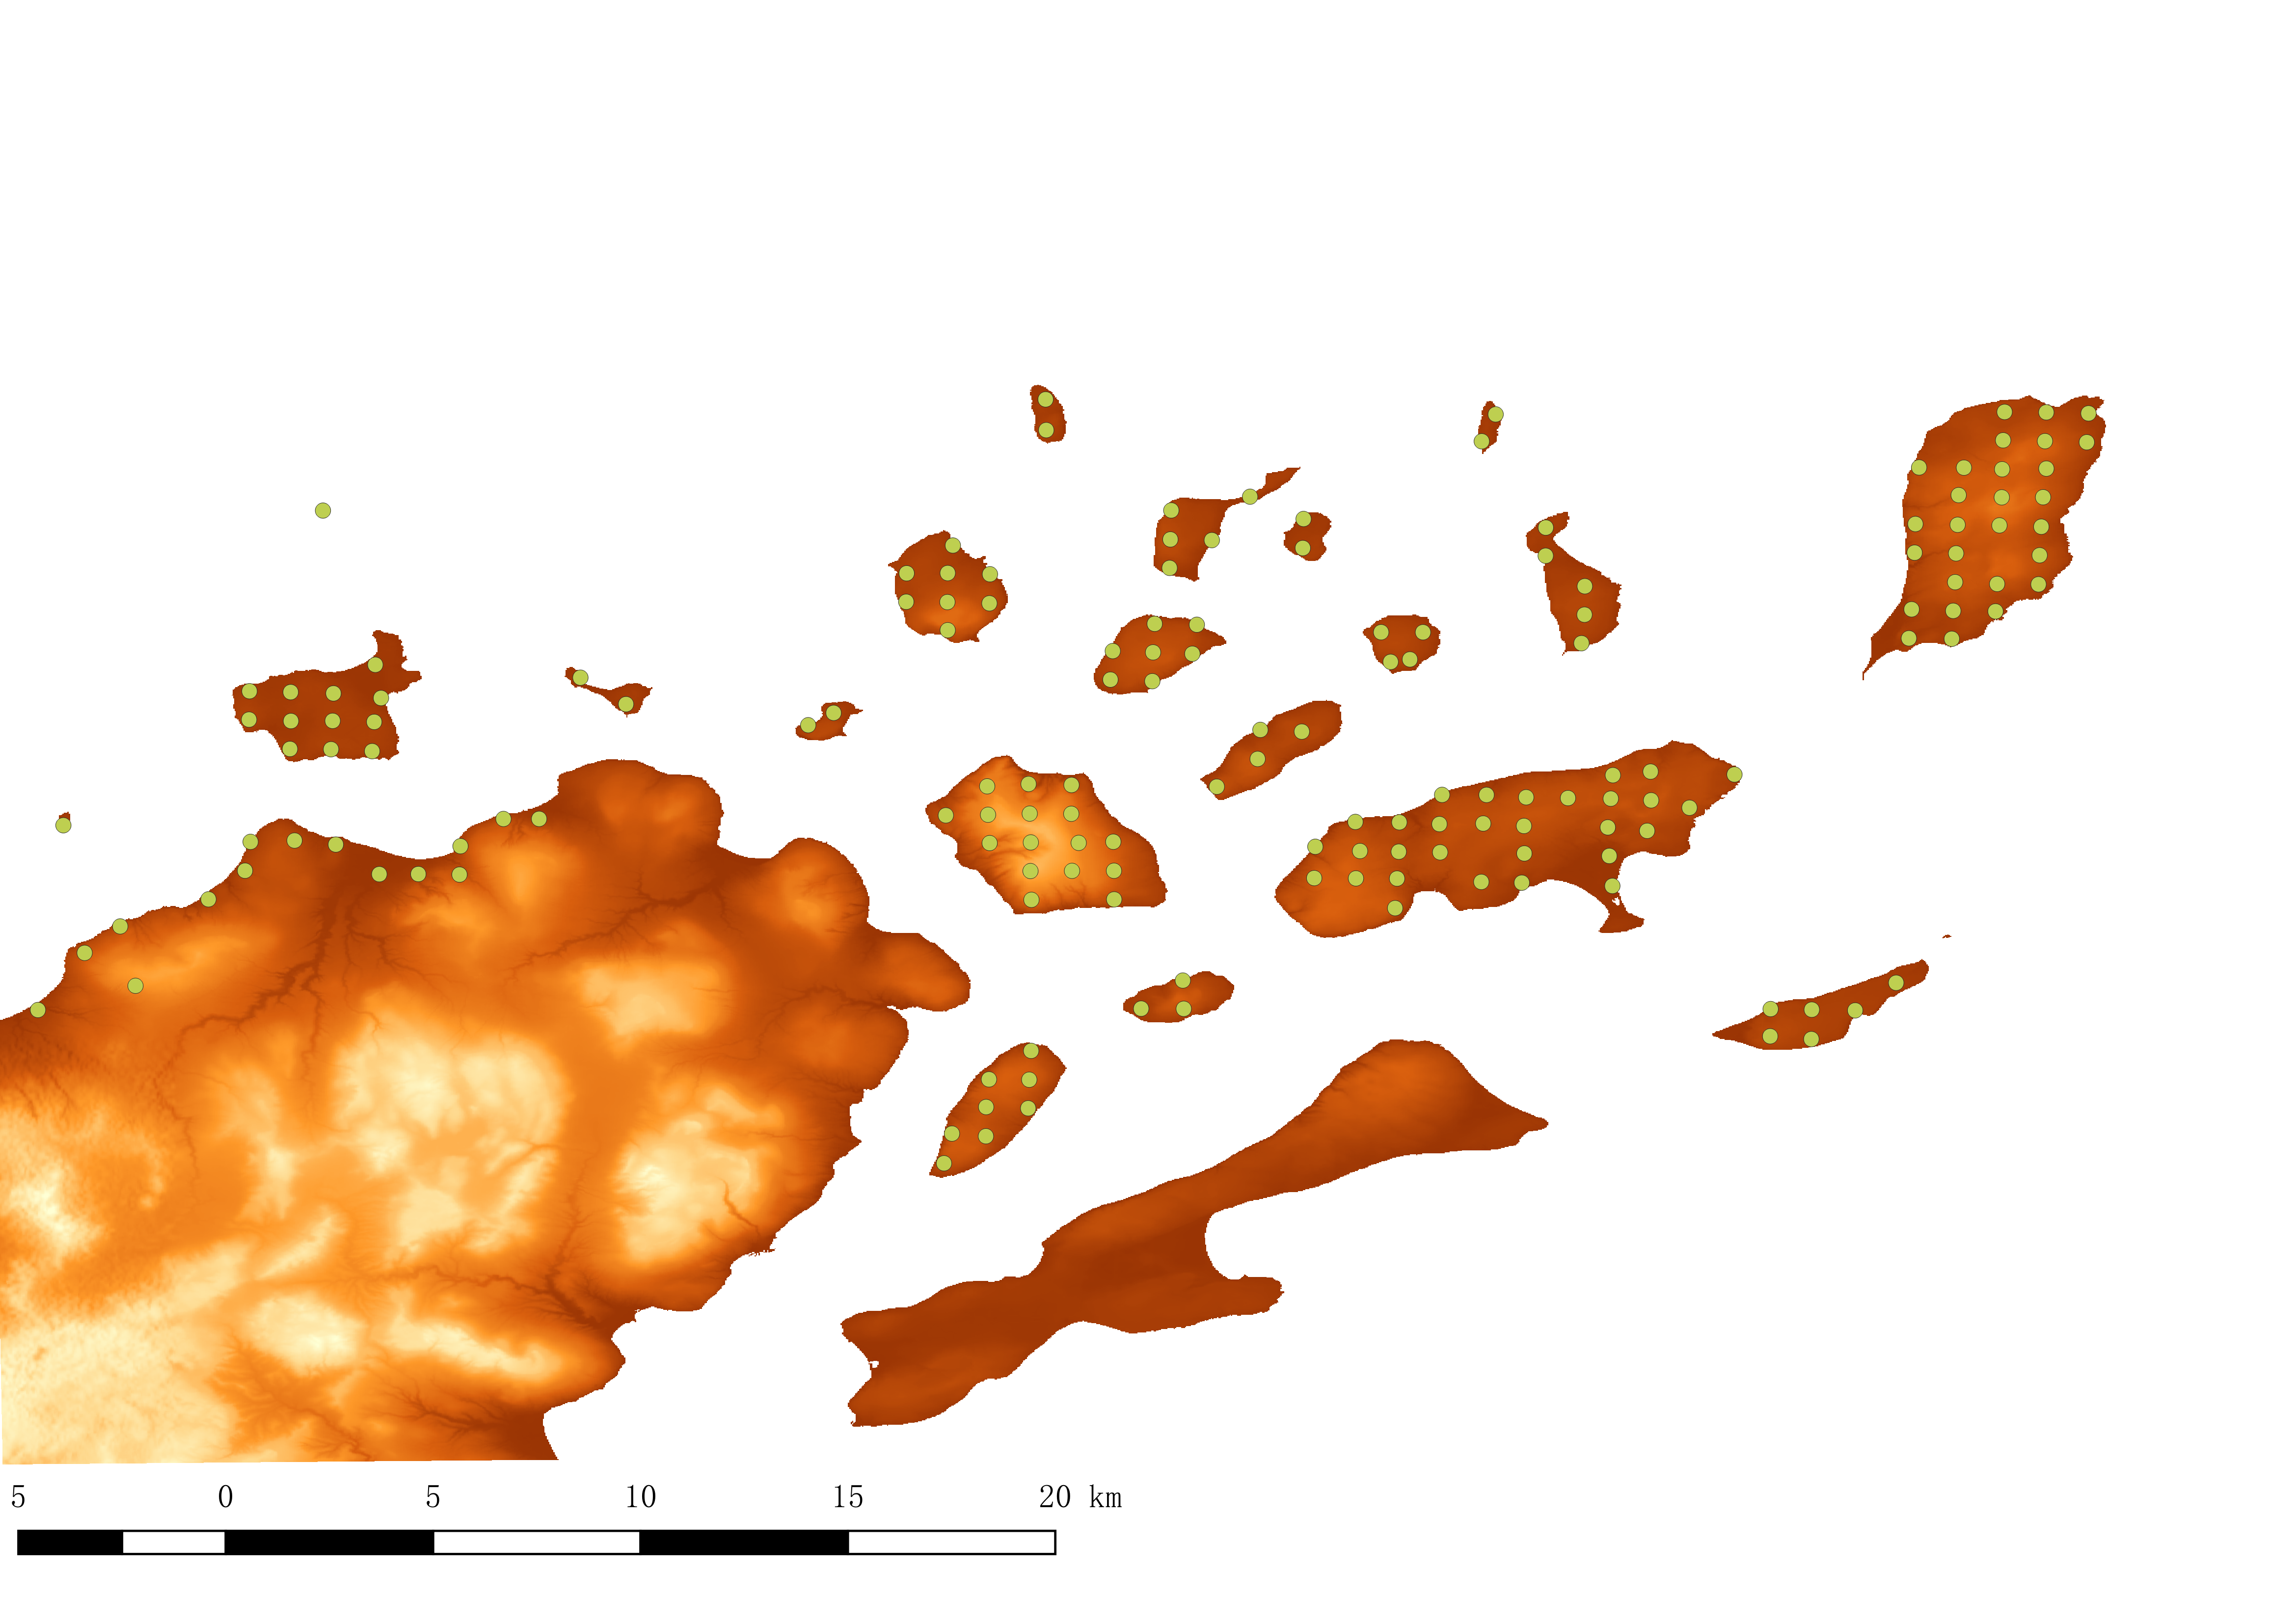
\includegraphics[scale=.3]{fig/APIS/APIS_camera.png}
		%\caption{Wilson}
		\label{beta-size}
	\end{figure}
\end{frame}

\begin{frame}{Simple Test on $\beta$-diversity}
	\begin{columns}[c]
		\column{7cm}
		\begin{figure}[ht]
			\centering
			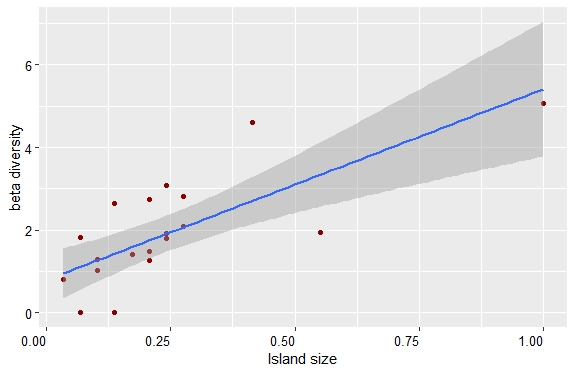
\includegraphics[scale=.5]{fig/APIS/beta_size.jpeg}
			%\caption{Wilson}
			\label{beta-size}
		\end{figure}
		
		\column{4cm}
		\begin{itemize}
			\item $\beta$-diversity roughly tells us the spatial structure of diversity
			\item Larger island has richer spatial structure (p=1.71e-4, adj-$R^{2}$=0.53)
		\end{itemize}
	\end{columns}
\end{frame}

\begin{frame}{Exchangable Approximation of Species}
\begin{itemize}
	\item Species are similar\pause
	\item Is it appropriate? \\Context dependent!
\end{itemize}
\end{frame}




\begin{frame}{Resources and Species Similarity}
	\begin{itemize}
		\item Lots of island research are in tropical area with rich resources
		\item What about Apostles?
		\begin{itemize}
			\item[]
			\item[] 
		\end{itemize}
	\end{itemize}
\end{frame}

\begin{frame}{Apostle Islands Climate} % talk about specific speices.
	\begin{figure}[ht]
		\centering
		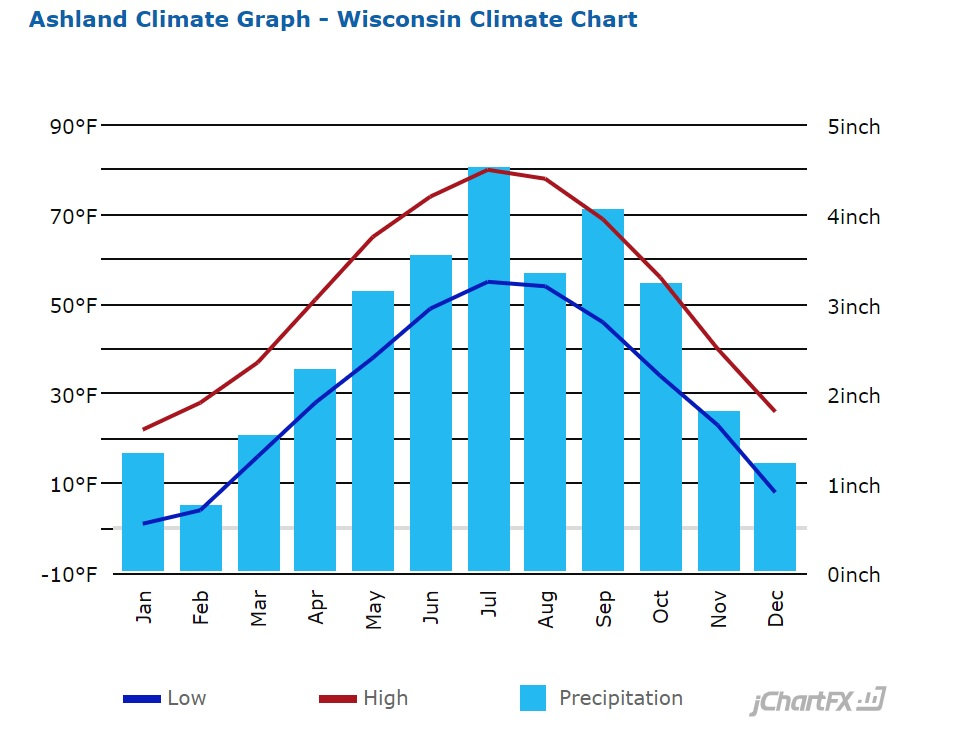
\includegraphics[scale=.6]{fig/APIS/climate.jpg}
		%\caption{Wilson}
		\label{climate}
	\end{figure}
\end{frame}

\begin{frame}{Resources and Species Similarity}
	\begin{itemize}
		\item Lots of island research are in tropical area with rich resources
		\item What about Apostles?\pause
		\begin{itemize}
			\item Temperate area, less resources
			\item Harsh winter 
		\end{itemize}
	\end{itemize}
\end{frame}

\begin{frame}{Big Questions}
	How do we distinguish different signals from distribution and evaluate the contribution between:
	\begin{itemize}
		\item Environmental sorting
		\item Direct Interactions (e.g. exclusion)
		\item Spatial Auto-correlation 
	\end{itemize}
\end{frame}

\begin{frame}{Explicit Modeling Needed}
	\begin{itemize}
		\item Both inter and intra island spatial relationships
		\item Interspecific relationships
		\item So that we can compare different processes' contribution!
	\end{itemize}
\end{frame}

\begin{frame}{More Specific Question}
	Spatial and competition, which has the strongest influence on canid's distribution on APIS?
\end{frame}


\subsection{Markov Random Field}
%\begin{frame}{How do We Model Network?}
%	Graphical Modeling!
%\end{frame}
\begin{frame}{Representing Relationships, Graph}
	\begin{columns}
		\column{.5\textwidth}
		\begin{block}{Directed Graph}
			\begin{figure}[ht]
				\centering
				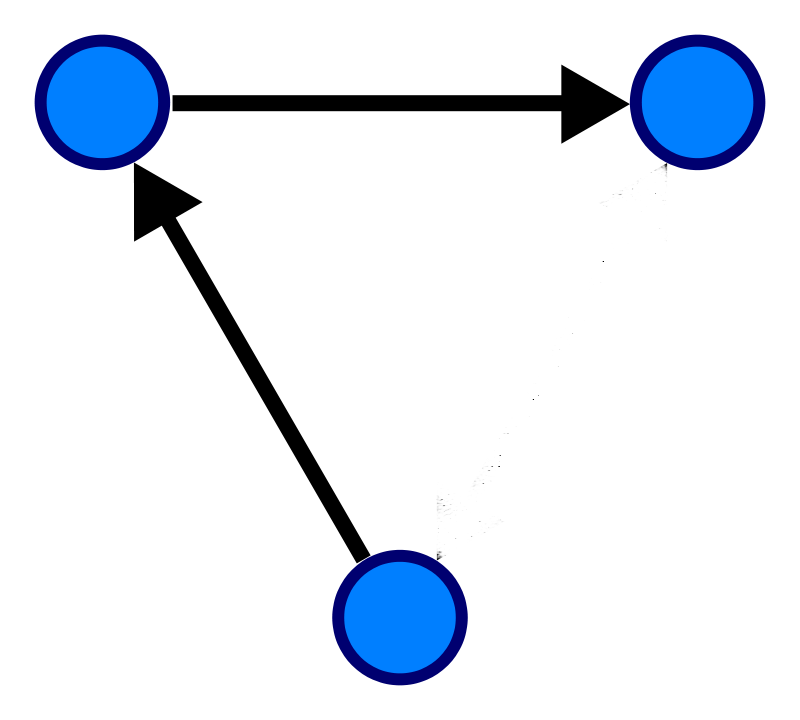
\includegraphics[scale=0.18]{fig/APIS/Directed1.png}
				%\caption{}
				\label{DG}
			\end{figure}
		\end{block}
		
		\column{.5\textwidth}
		\begin{block}{Undirected Graph}
			\begin{figure}[ht]
				\centering
				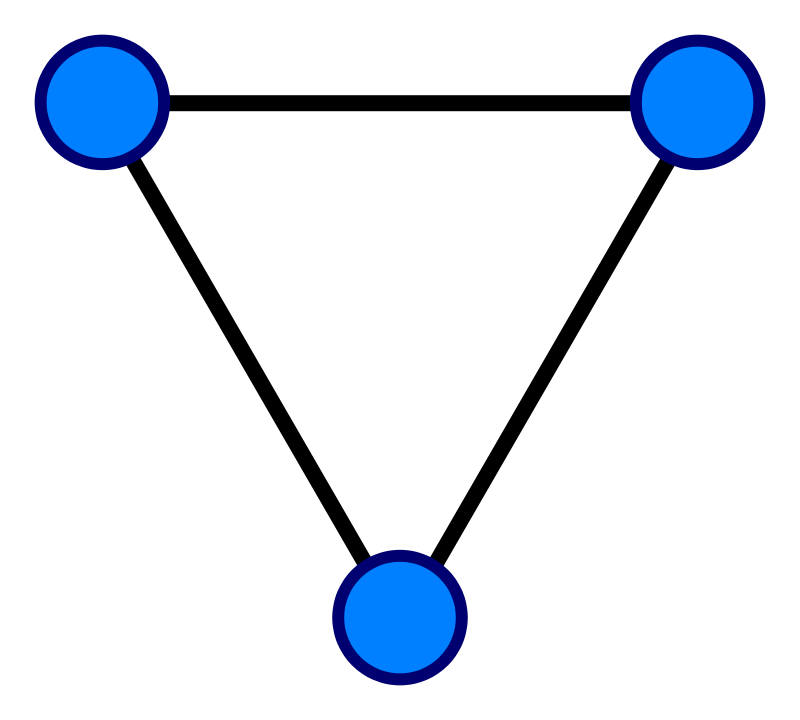
\includegraphics[scale=0.18]{fig/APIS/Undirected.png}
				%\caption{Wilson}
				\label{UDG}
			\end{figure}
		\end{block}
		
	\end{columns}
\end{frame}

\begin{frame}{Probabilistic Graph Model}
	\begin{itemize}
		\item Vertices are random variables (in our case, presence/absence of a certain species at certain microsite)
		\item Edges are correlations or conditional
		\item PGM for different graph:
		\begin{itemize}
			\item Bayesian Network: Directed (Acyclic)
			\item \textbf{Markov Random Field}: Undirected
		\end{itemize}
	\end{itemize}
\end{frame}

\begin{frame}{Why MRF}
	\begin{itemize}
		\item Allow \textit{cycles}: e.g. a-b-c-a was allowed in MRF but not BN
		\item Undirected nature of spatial autocorrelation and niche overlap
		\item Defines an Energy
	\end{itemize}
\end{frame}

\begin{frame}{A Conceptual Example: 2 Islands and 2 Species}
	\begin{figure}[ht]
		\centering
		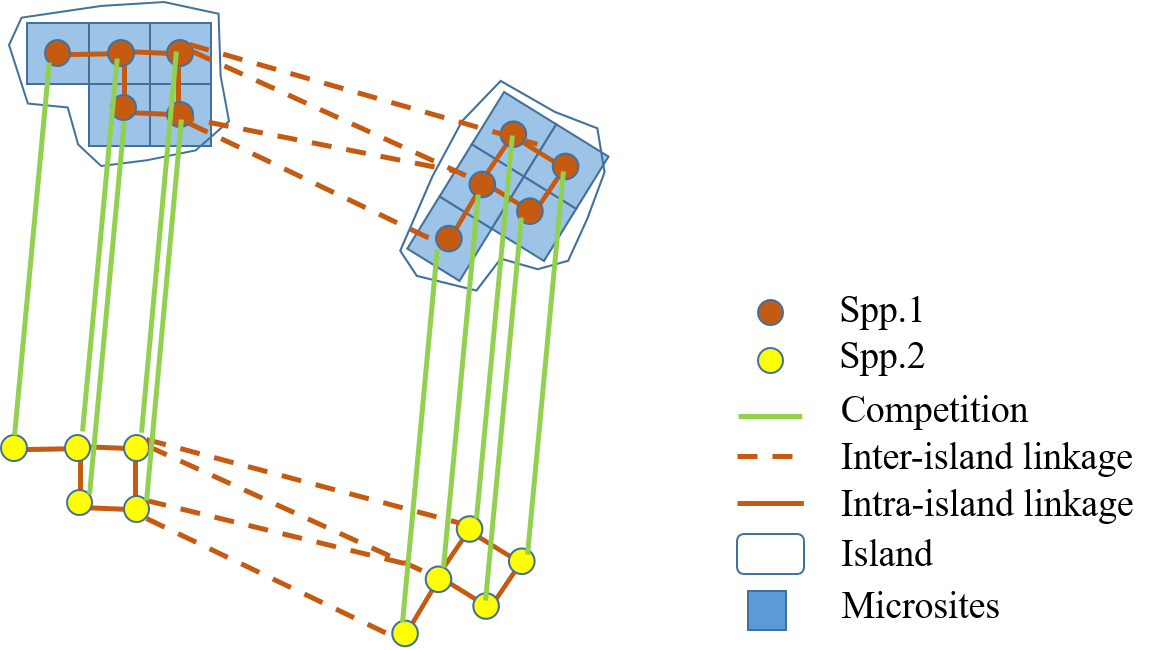
\includegraphics[scale=.4]{fig/APIS/sample_graph.png}
		%\caption{Wilson}
		\label{sample_graph}
	\end{figure}
\end{frame}

\section{Methods}
\begin{frame}{Method}
	\begin{itemize}
		\item MRF of Apostle Island
	\end{itemize}
\end{frame}

\subsection{MRF of Apostle Islands} %  Formalization of the model, how to assign the graph, 

\begin{frame}{Microsite Linkage: Delaunay Triangle}
	\begin{figure}[t]
		%\centering
		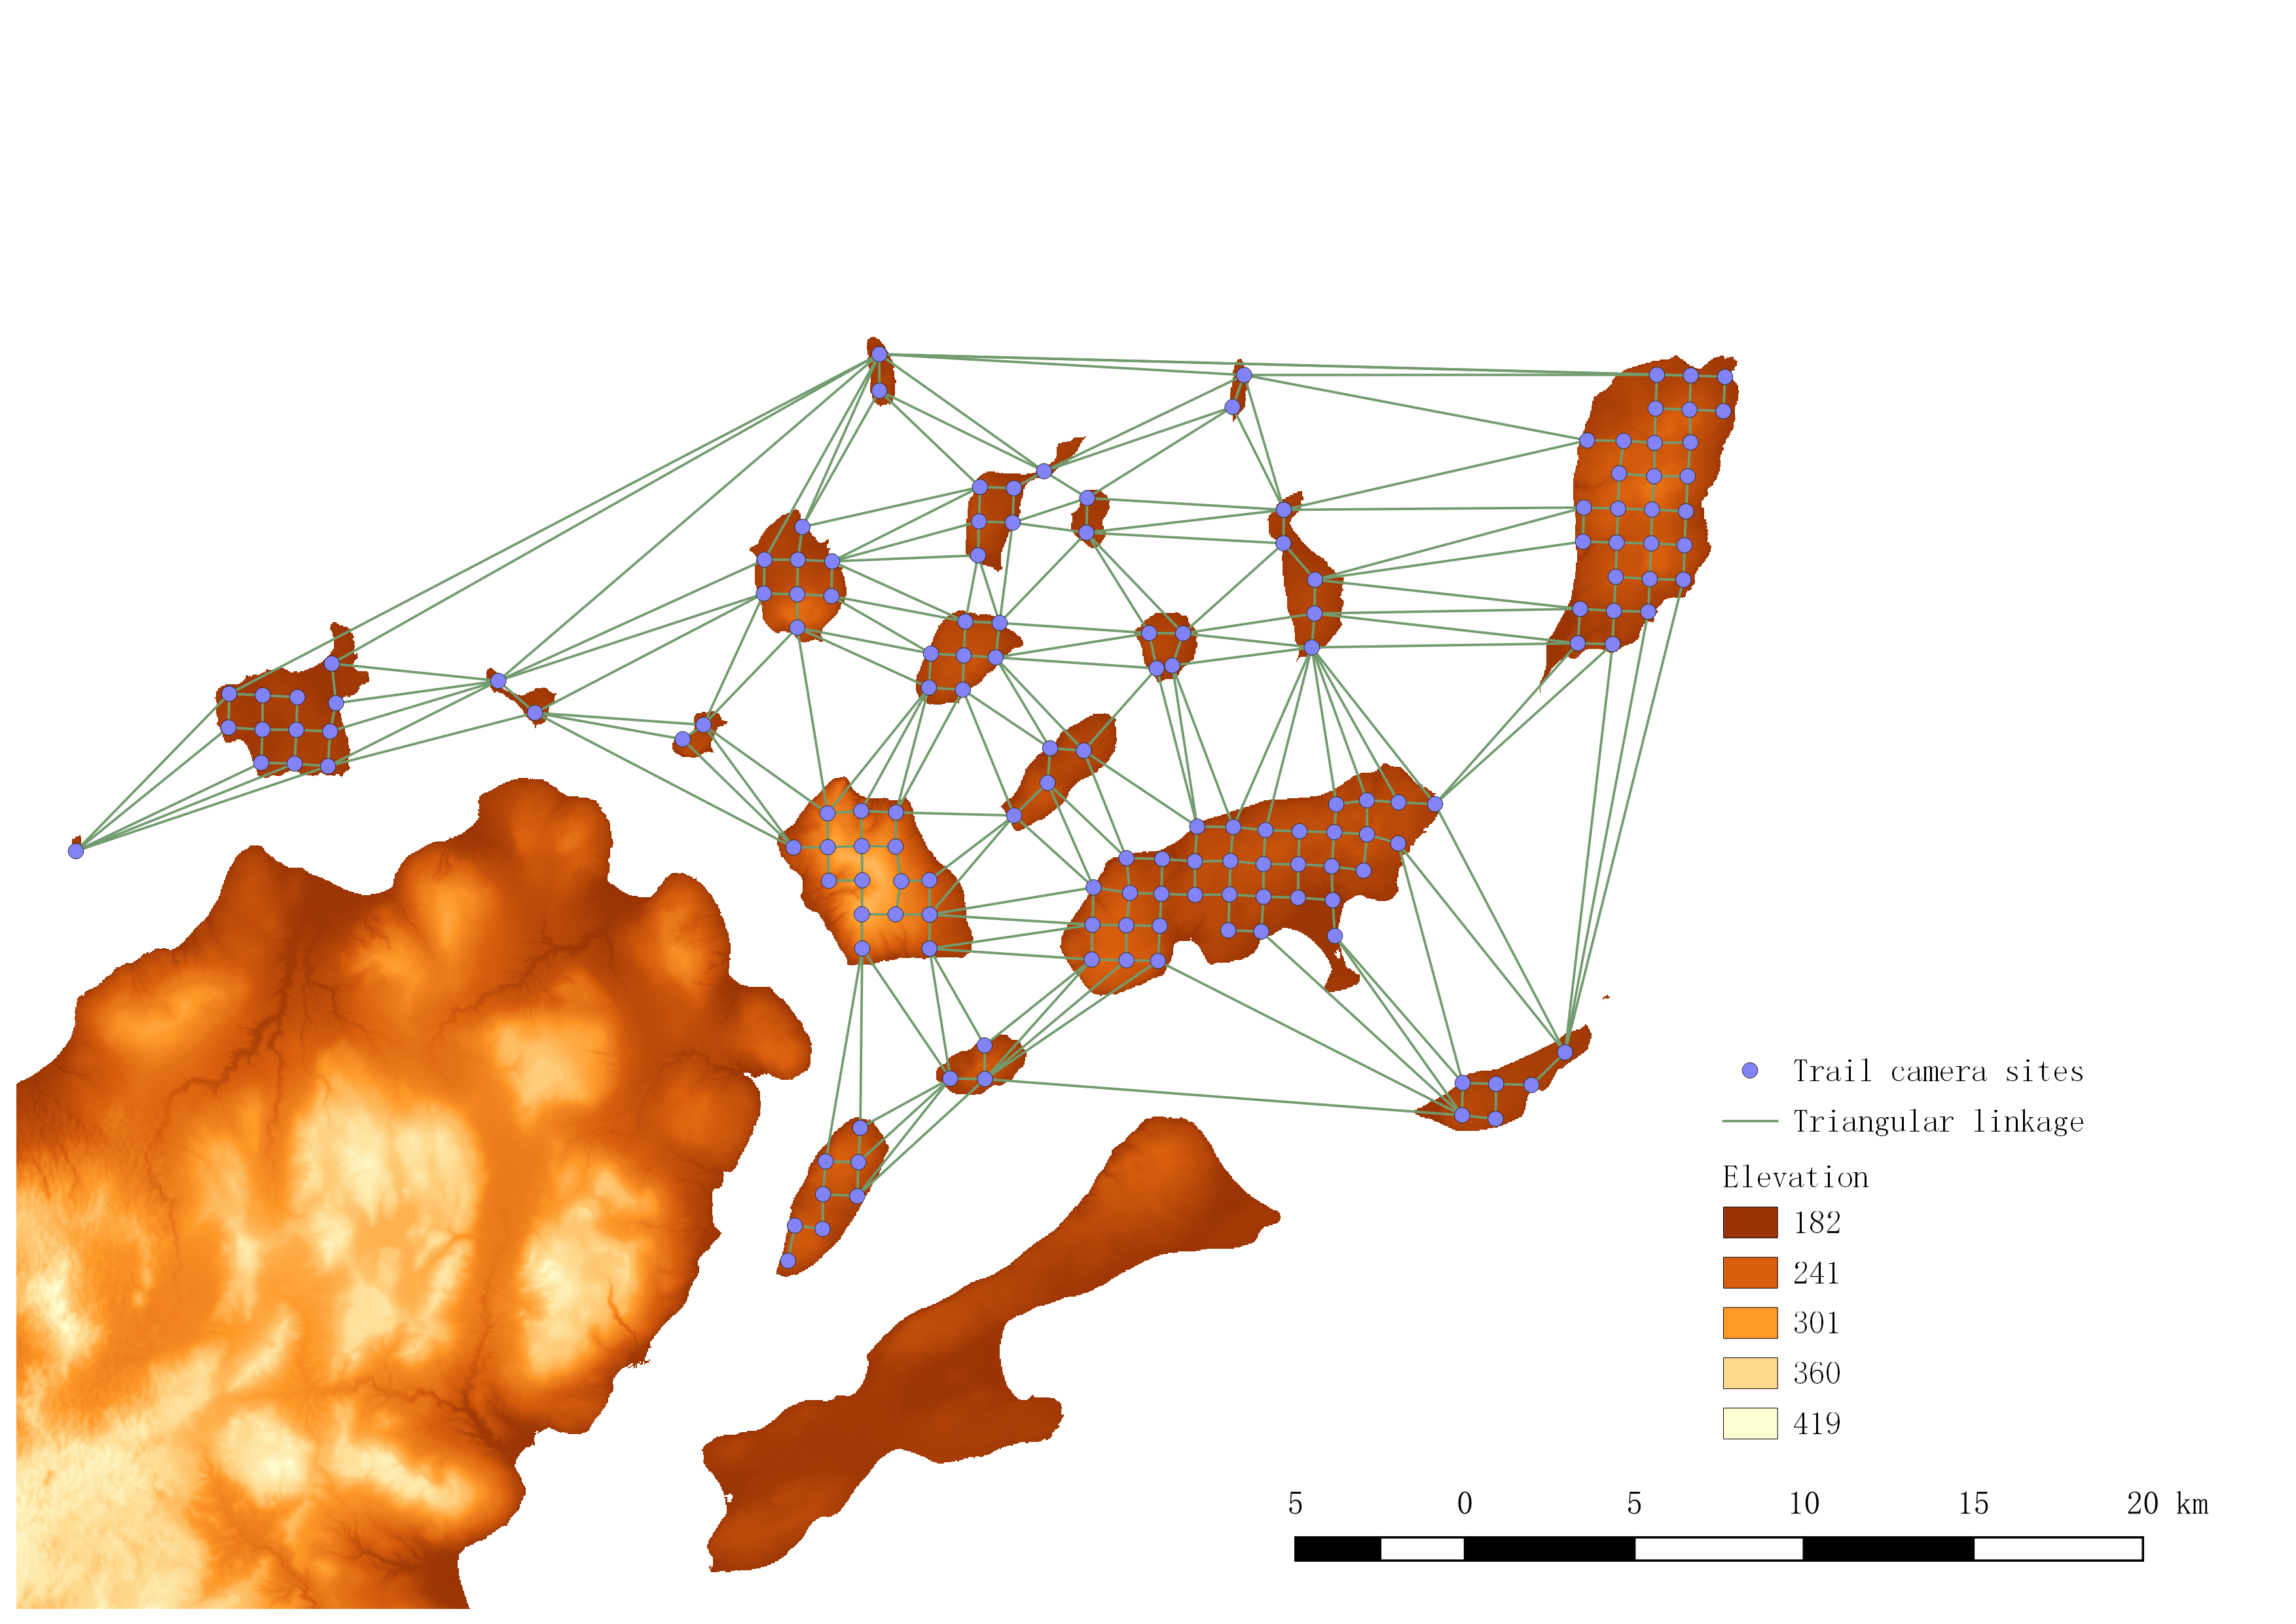
\includegraphics[scale=0.28]{fig/APIS/APIS_graph.png}
		\caption{Site Linkage of APIS}
		\label{fig_graph}
	\end{figure}
\end{frame} 
% more graphical of demes.

\begin{frame}{Mainland Linkage}
	\begin{itemize}
		\item If a site has mainland as its nearest interisland linkage, it is linked to mainland.
	\end{itemize}
\end{frame}

\subsection{Formalization}
\begin{frame}{Modeling Pattern as Pattern}
	\begin{itemize}
		\item Distribution pattern should be view as a random vector, for S sites and w species, it is $S\times w$ dimensional vector
		\[
		\mathbf{Z}=(Z_{1}^{1},Z_{1}^{2}...Z_{2}^{1},Z_{2}^{2},...Z_{i}^{l}...Z_{S}^{w})^{T}\in \{-1,+1\}^{Sw}
		\]
		\item An example for 2 species and 2 sites:
		\[
		\mathbf{Z}=(+1,-1,-1,+1)^{T}
		\]
		Spp1 occurs on site 1 but not 2, spp2 occurs on site 2 but not 1
	\end{itemize}
\end{frame}

\begin{frame}{Markov Random Field: Probability of a Certain Distribution Pattern}
\begin{itemize}
	\item Probability of pattern $\mathbf{Z}$ is given by
	\begin{equation}
	\begin{aligned}
	P(\mathbf{Z}|\theta)\propto &exp[ \sum_{k=1}^{w} (\mathbf{X}\beta_{k} \mathbf{Z}_{k}\\ 
	&+ \frac{1}{2}\mathbf{Z}_{k}^{T}\mathbf{D}_{k}^{in}\mathbf{Z}_{k}\\
	&+ \frac{1}{2}\mathbf{Z}_{k}^{T}\mathbf{D}_{k}^{ex}\mathbf{Z}_{k}\\
	&+ \sum_{l>k}\eta_{lk}\mathbf{Z}_{k}^{T}\mathbf{Z}_{l})]\\
	\end{aligned}
	\end{equation}
	\item $C(\theta)$ is called \textit{partition function} and is usually intractable
\end{itemize}
\end{frame}
% point out sepcific terms

\begin{frame}{MRF is an Energy Based Model}
	\begin{itemize}
		\item MRF defined an potential energy function (a.k.a. Hamiltonian in physics)
		\item Can be used to evaluate contribution of different terms
	\end{itemize}

\end{frame}

% parameterization and justification of the model, theoretical aspect, FI goes here
\subsection{Imperfect Observations}
\begin{frame}{Imperfect Observations}
	\begin{itemize}
		\item Infer detection probability from the detection history assuming occupancy won't change.
		\item Also contains inter-specific interaction but assumed to be local:
		\begin{equation}
		\begin{aligned}
			P(y_{1ij},y_{2ij},...|Z_{1i},Z_{2i},...)&\propto exp(\sum_{k=1}^{w}[\beta^{det}_{k}X^{det}_{ij}y_{kij}I_{Z_{ki}=1}\\
			&+\sum_{l> k}\delta_{kl}y_{kij}y_{lij}I_{Z_{ki}=1}I_{Z_{li}=1}])
		\end{aligned}	
		\end{equation}
	\end{itemize}
\end{frame}
%\subsection{Bayesian Inference} % Difficulties and Murray sampler
\begin{frame}{Bayesian Framework: Sampling from Posterior}
	\begin{itemize}
		\item This task is generally hard because of the \textit{partition function} (one cannot evaluate the likelihood!)
		\item I will use Murray 2014's parameter exchanging method to deal with this problem
	\end{itemize}
\end{frame}

\begin{frame}{Evaluating Different Interactions}
\begin{itemize}
	\item Habitat Selection Matrix:
	\begin{itemize}
		\item Evaluate the \textbf{landscape scale niche partitioning} of species
		\item I used covariance of linear predictors (a.k.a. external field)
		\item Positive means spp1 and spp2 has similar habitat selection in landscape scale
	\end{itemize}
	\pause
	\item Direct Association
	\begin{itemize}
		\item Evaluate \textbf{local direct association} between species that cannot be explained by environmental sorting
		\item Use the coupling matrix in MRF model
	\end{itemize}
	\pause
	\item Detection as measure of behavior
	\begin{itemize}
		\item Evaluate local direct association between \textbf{detection} that cannot be explained by environment
		\item Coupling matrix in detection MRF model
	\end{itemize}
\end{itemize}

\end{frame}

\section{Primary Results}
\begin{frame}{Primary Results}
	\begin{itemize}
		\item Fitting MRF of 2 simulated species
		\begin{itemize}
			\item 4 repeats
			\item False-negative
		\end{itemize}
		\item Real Case Studies
		\begin{itemize}
			\item Island System
			\begin{itemize}
				\item Fisher-Marten
				\item Coyote-Fox-Bobcat
			\end{itemize}
			
			\item Mountain System
			\begin{itemize}
				\item Leopardcat-Civet-Marten
				\item Muskdeer-Tuftsdeer-Muntjac 
			\end{itemize}
			
		\end{itemize}
	\end{itemize}
\end{frame}
\subsection{Fitting a APIS MRF of 2 Simulated Species}
\begin{frame}{Simulated Distribution Pattern}
	\begin{columns}
		\column{6cm}
		\begin{figure}[ht]
			\centering
			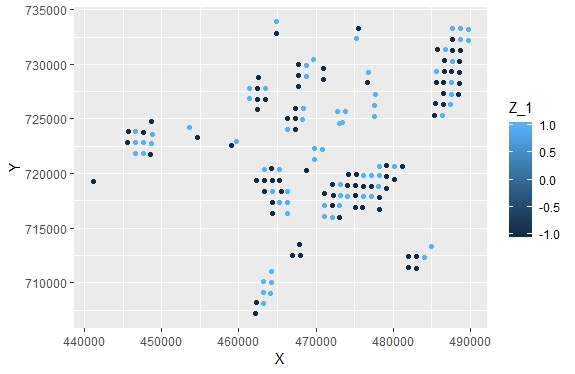
\includegraphics[scale=.4]{fig/Island_2spp/Z1.jpeg}
			%\caption{Wilson}
			\label{Z1}
		\end{figure}
		\column{6cm}
		\begin{figure}[ht]
			\centering
			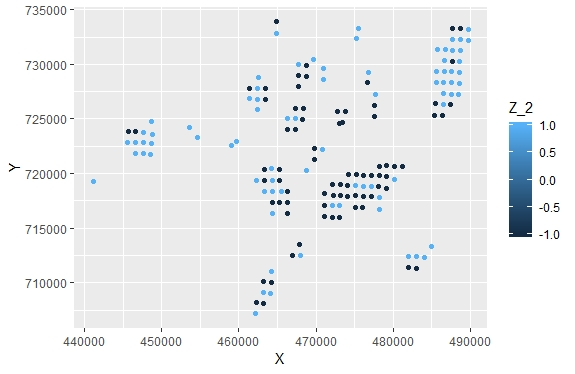
\includegraphics[scale=.4]{fig/Island_2spp/Z2.jpeg}
			%\caption{Wilson}
			\label{Z2}
		\end{figure}
		
	\end{columns}
\end{frame}

\begin{frame}{Fitting Parameters}
		\begin{columns}
		\column{6cm}
		\begin{figure}[ht]
			\centering
			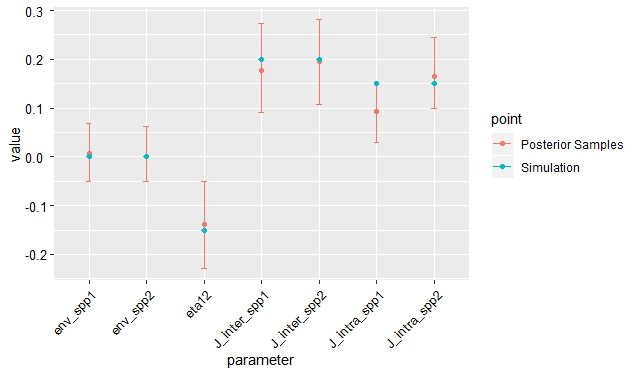
\includegraphics[scale=.4]{fig/Island_2spp/occu.jpeg}
			%\caption{Wilson}
			\label{occu}
		\end{figure}
		\column{6cm}
		\begin{figure}[ht]
			\centering
			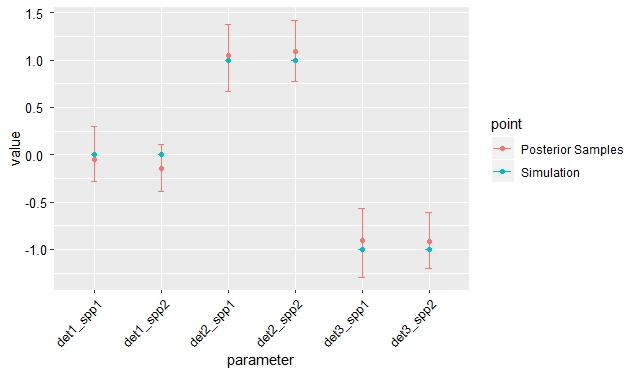
\includegraphics[scale=.4]{fig/Island_2spp/det.jpeg}
			%\caption{Wilson}
			\label{det}
		\end{figure}
		
	\end{columns}
	
\end{frame}

\subsection{Fisher and Marten System}
\begin{frame}{APIS, Two Systems Tested}
	\begin{itemize}
		\item Fisher-Marten
		\item Coyote-Fox-Bobcat
	\end{itemize}
\end{frame}

\begin{frame}{Fisher-Marten: Direct Association}
\begin{figure}[ht]
			\centering
			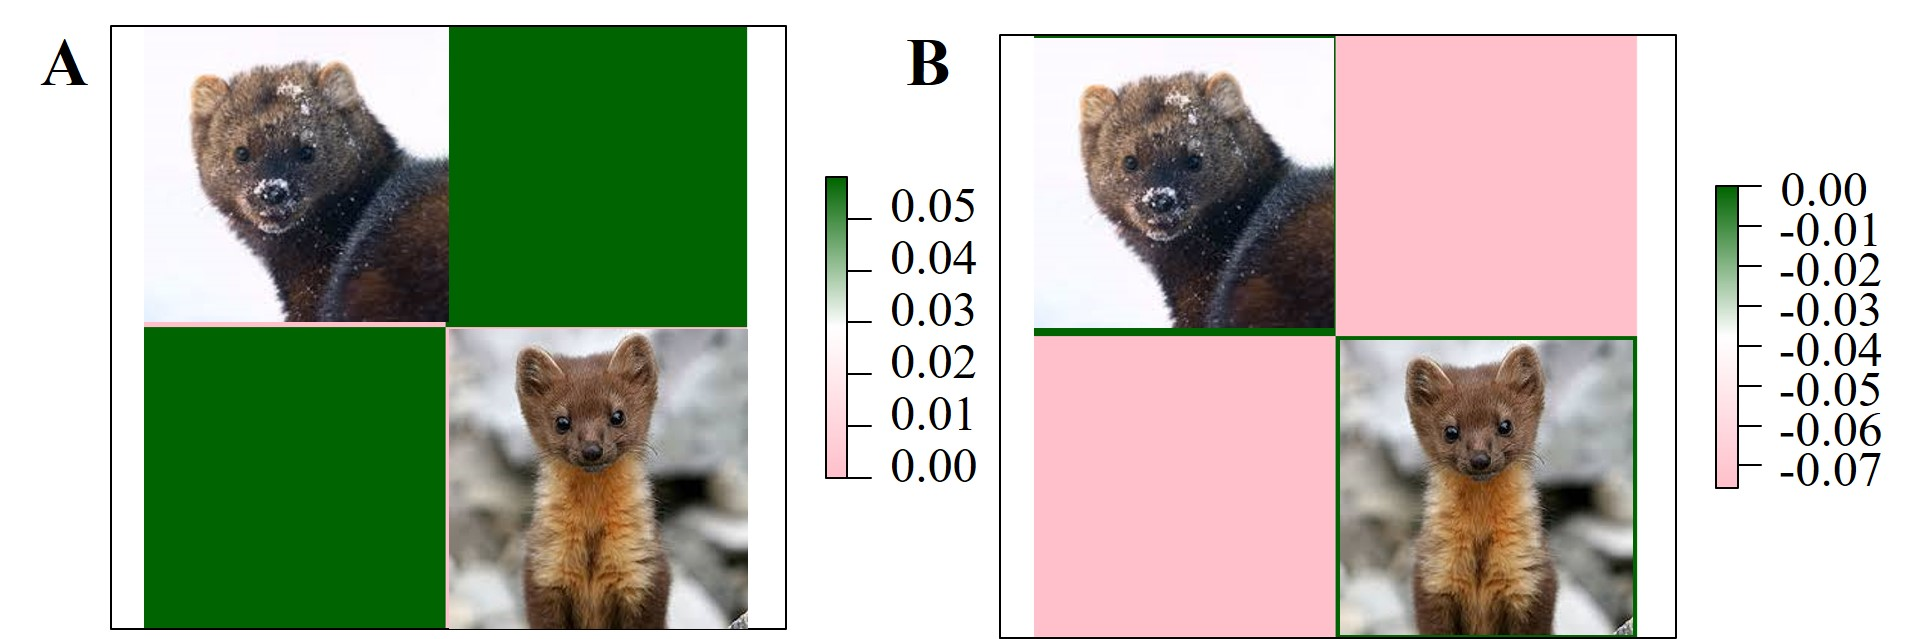
\includegraphics[scale=.35]{fig/APIS/FM/FM.jpg}
			%\caption{Wilson}
			\label{FM}
		\end{figure}
\end{frame}


\begin{frame}{Fisher-Marten: Evaluate Contribution}
\begin{figure}[ht]
			\centering
			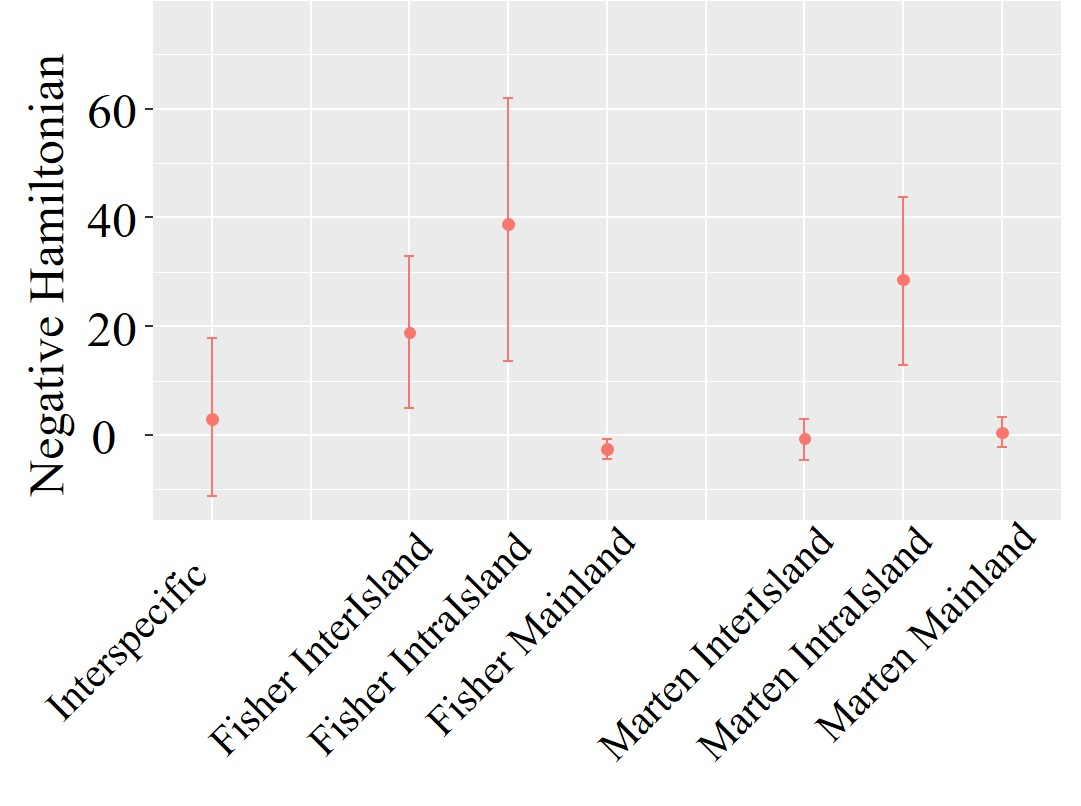
\includegraphics[scale=.4]{fig/APIS/FM/FM_Hamiltonian.jpg}
			%\caption{Wilson}
			\label{FM_H	}
\end{figure}
\end{frame}

\subsection{Coyote Fox Bobcat System}
\begin{frame}{Coyote Fox Bobcat: Direct Association}
\begin{figure}[ht]
			\centering
			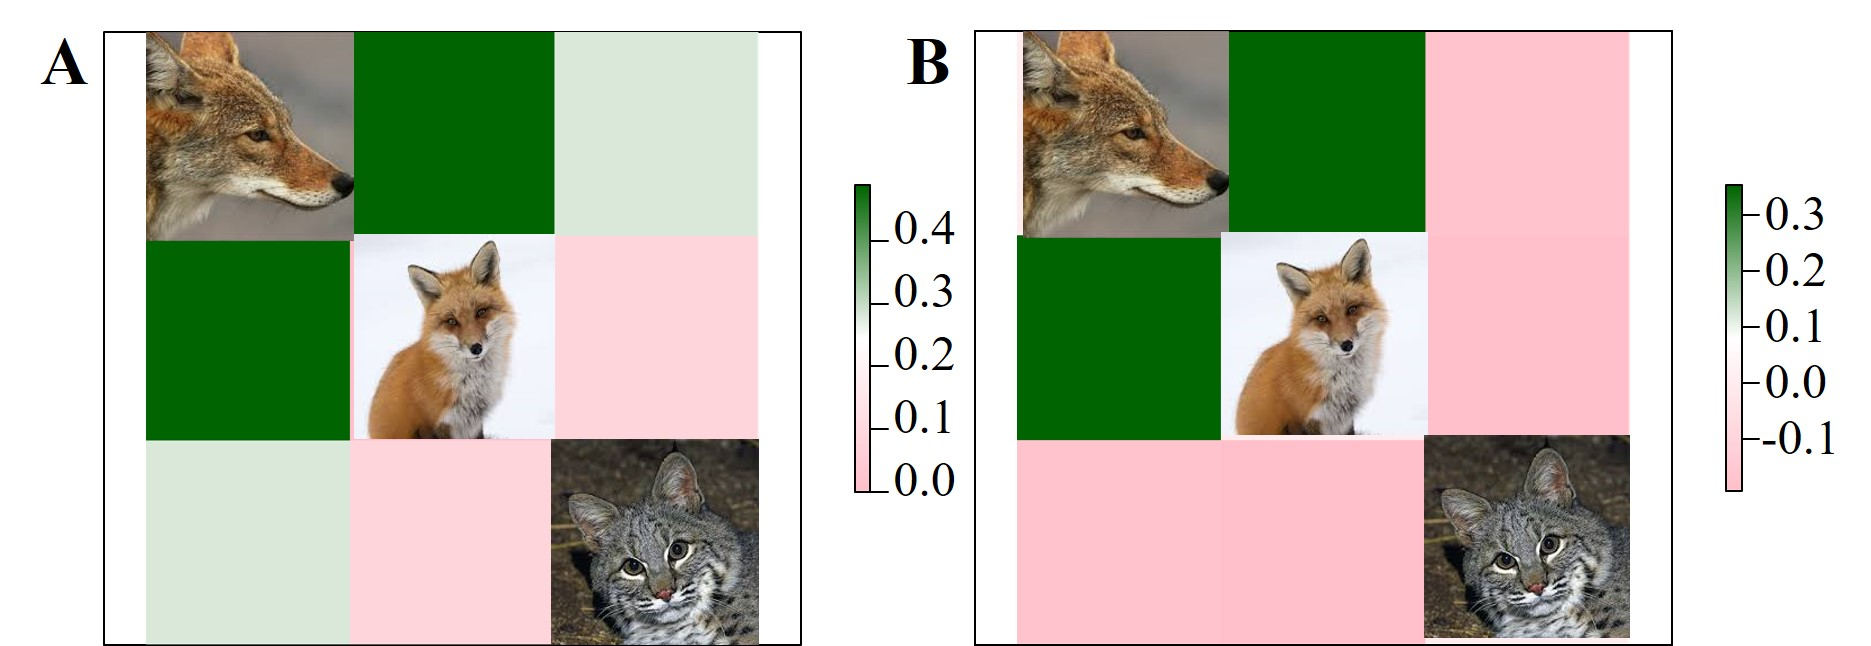
\includegraphics[scale=.35]{fig/APIS/CFB/CFB.jpg}
			%\caption{Wilson}
			\label{CFB}
		\end{figure}
\end{frame}


\begin{frame}{Coyote Fox Bobcat: Evaluate Contribution}
\begin{figure}[ht]
			\centering
			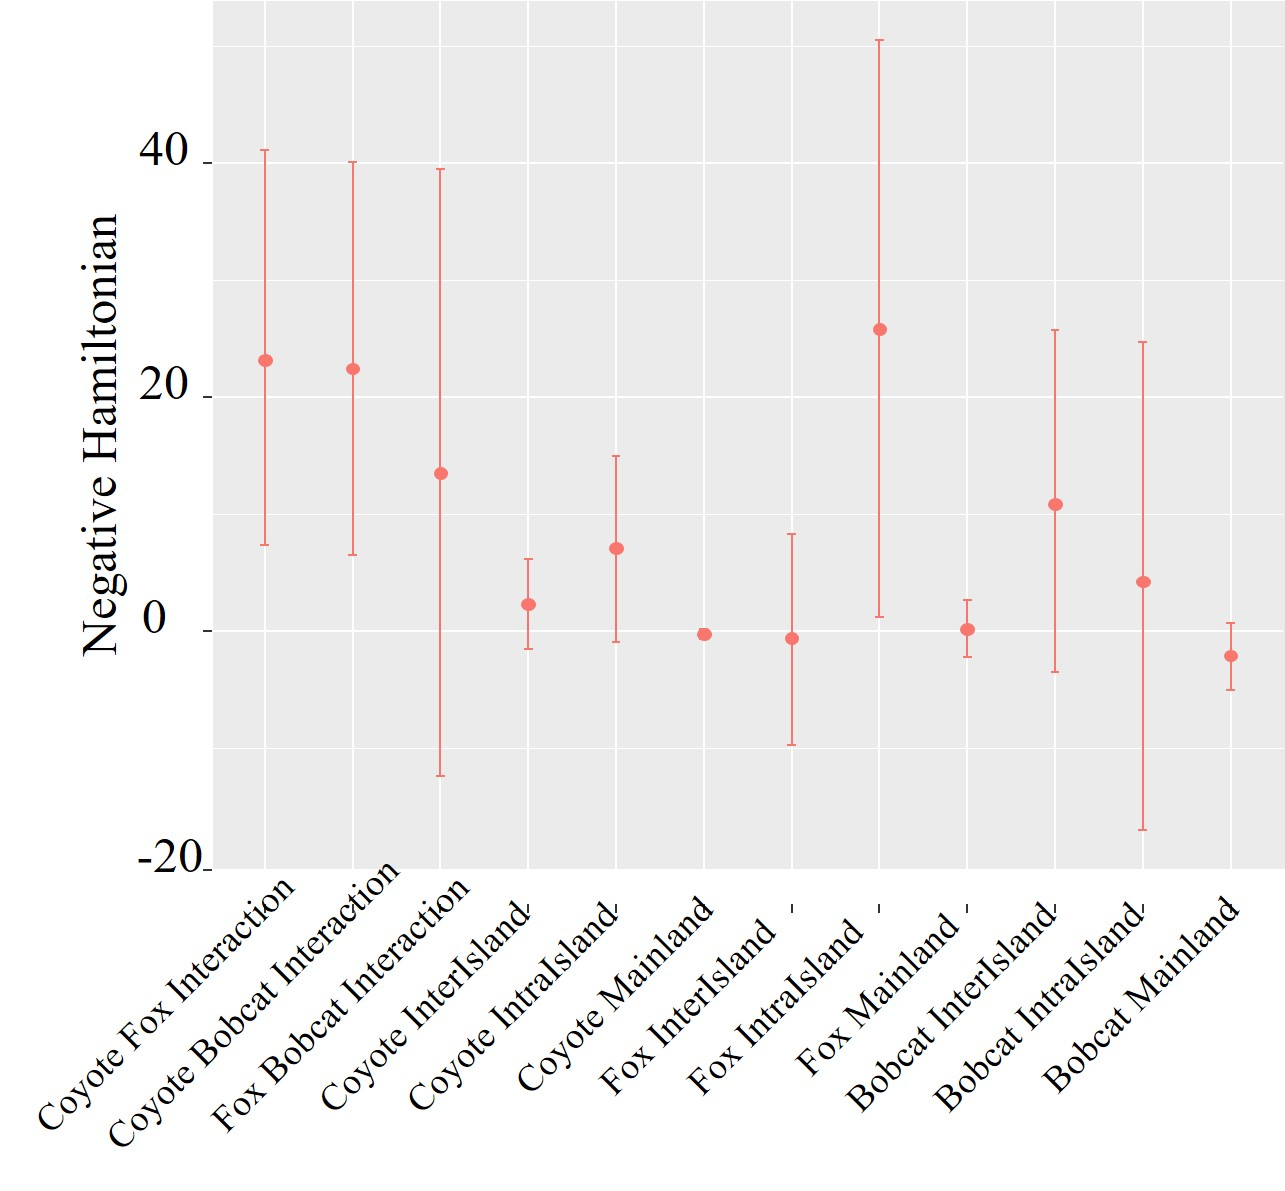
\includegraphics[scale=.3]{fig/APIS/CFB/CFB_Hamiltonian.jpg}
			%\caption{Wilson}
			\label{CFB_H	}
		\end{figure}
\end{frame}

\subsection{TJH: Land Systems with Elevation Gradient}
\begin{frame}{Two Distinct System}
	\begin{itemize}
		\item Carnivore: Leopardcat-Civet-Marten
		\item Herbivore: Muskdeer-Tuftsdeer-Muntjac 
	\end{itemize}
\end{frame}

\begin{frame}{Carnivore: Interaction Matrices}
	\begin{figure}[ht]
		\centering
		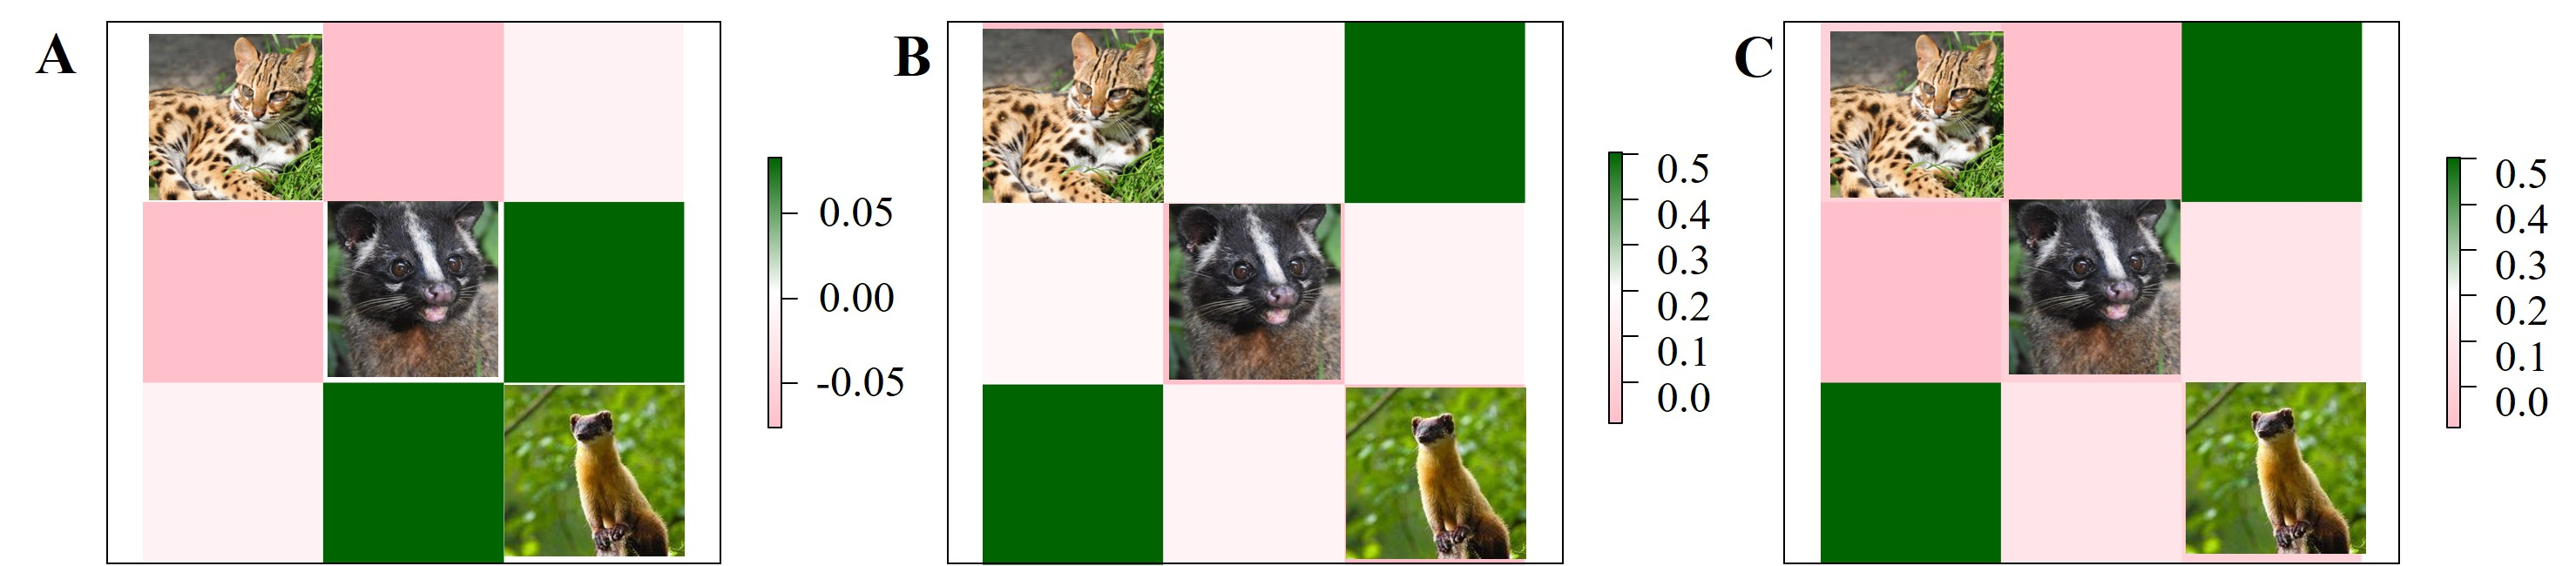
\includegraphics[scale=.23]{fig/TJH/car/TJH_carn.jpg}
		%\caption{Wilson}
		\label{carn}
	\end{figure}
\end{frame}

\begin{frame}{Herbivore: Interaction Matrices}
	\begin{figure}[ht]
		\centering
		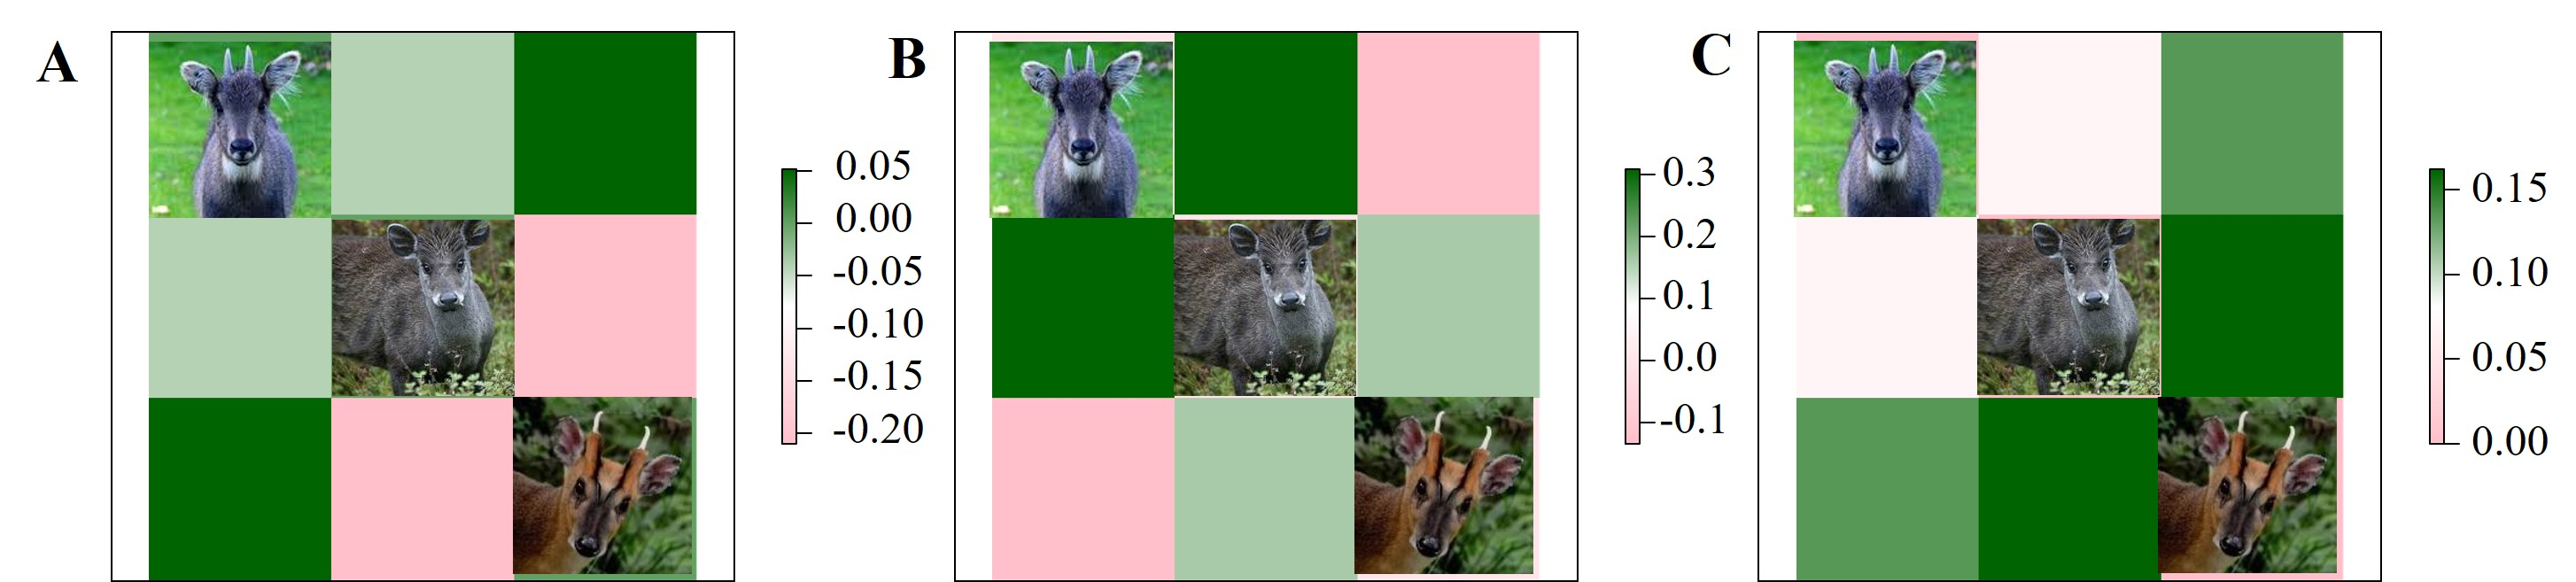
\includegraphics[scale=.23]{fig/TJH/herb/TJH_herb.jpg}
		%\caption{Wilson}
		\label{herb}
	\end{figure}
\end{frame}


\section{Initial Discussion}

\section{Next Steps \& Questions}

\begin{frame}{Next Step}
\begin{itemize}
	\item Model selection based on DIC
	\item Model evaluation
	\item Snapshot WI data
\end{itemize}
\end{frame}


\begin{frame}
	\huge{Questions and Comments are Welcomed!}
\end{frame}

\begin{frame}
	\Huge{Thank you}
\end{frame}

\end{document}